\documentclass[border=10pt]{standalone}
\usepackage[svgnames]{xcolor}
\usepackage{amsmath}
\usepackage{pgfplots}
\pgfplotsset{compat=newest}
\usepackage[sfdefault]{FiraSans}
\usepackage{FiraMono}
\renewcommand*\familydefault{\sfdefault}
\begin{document}
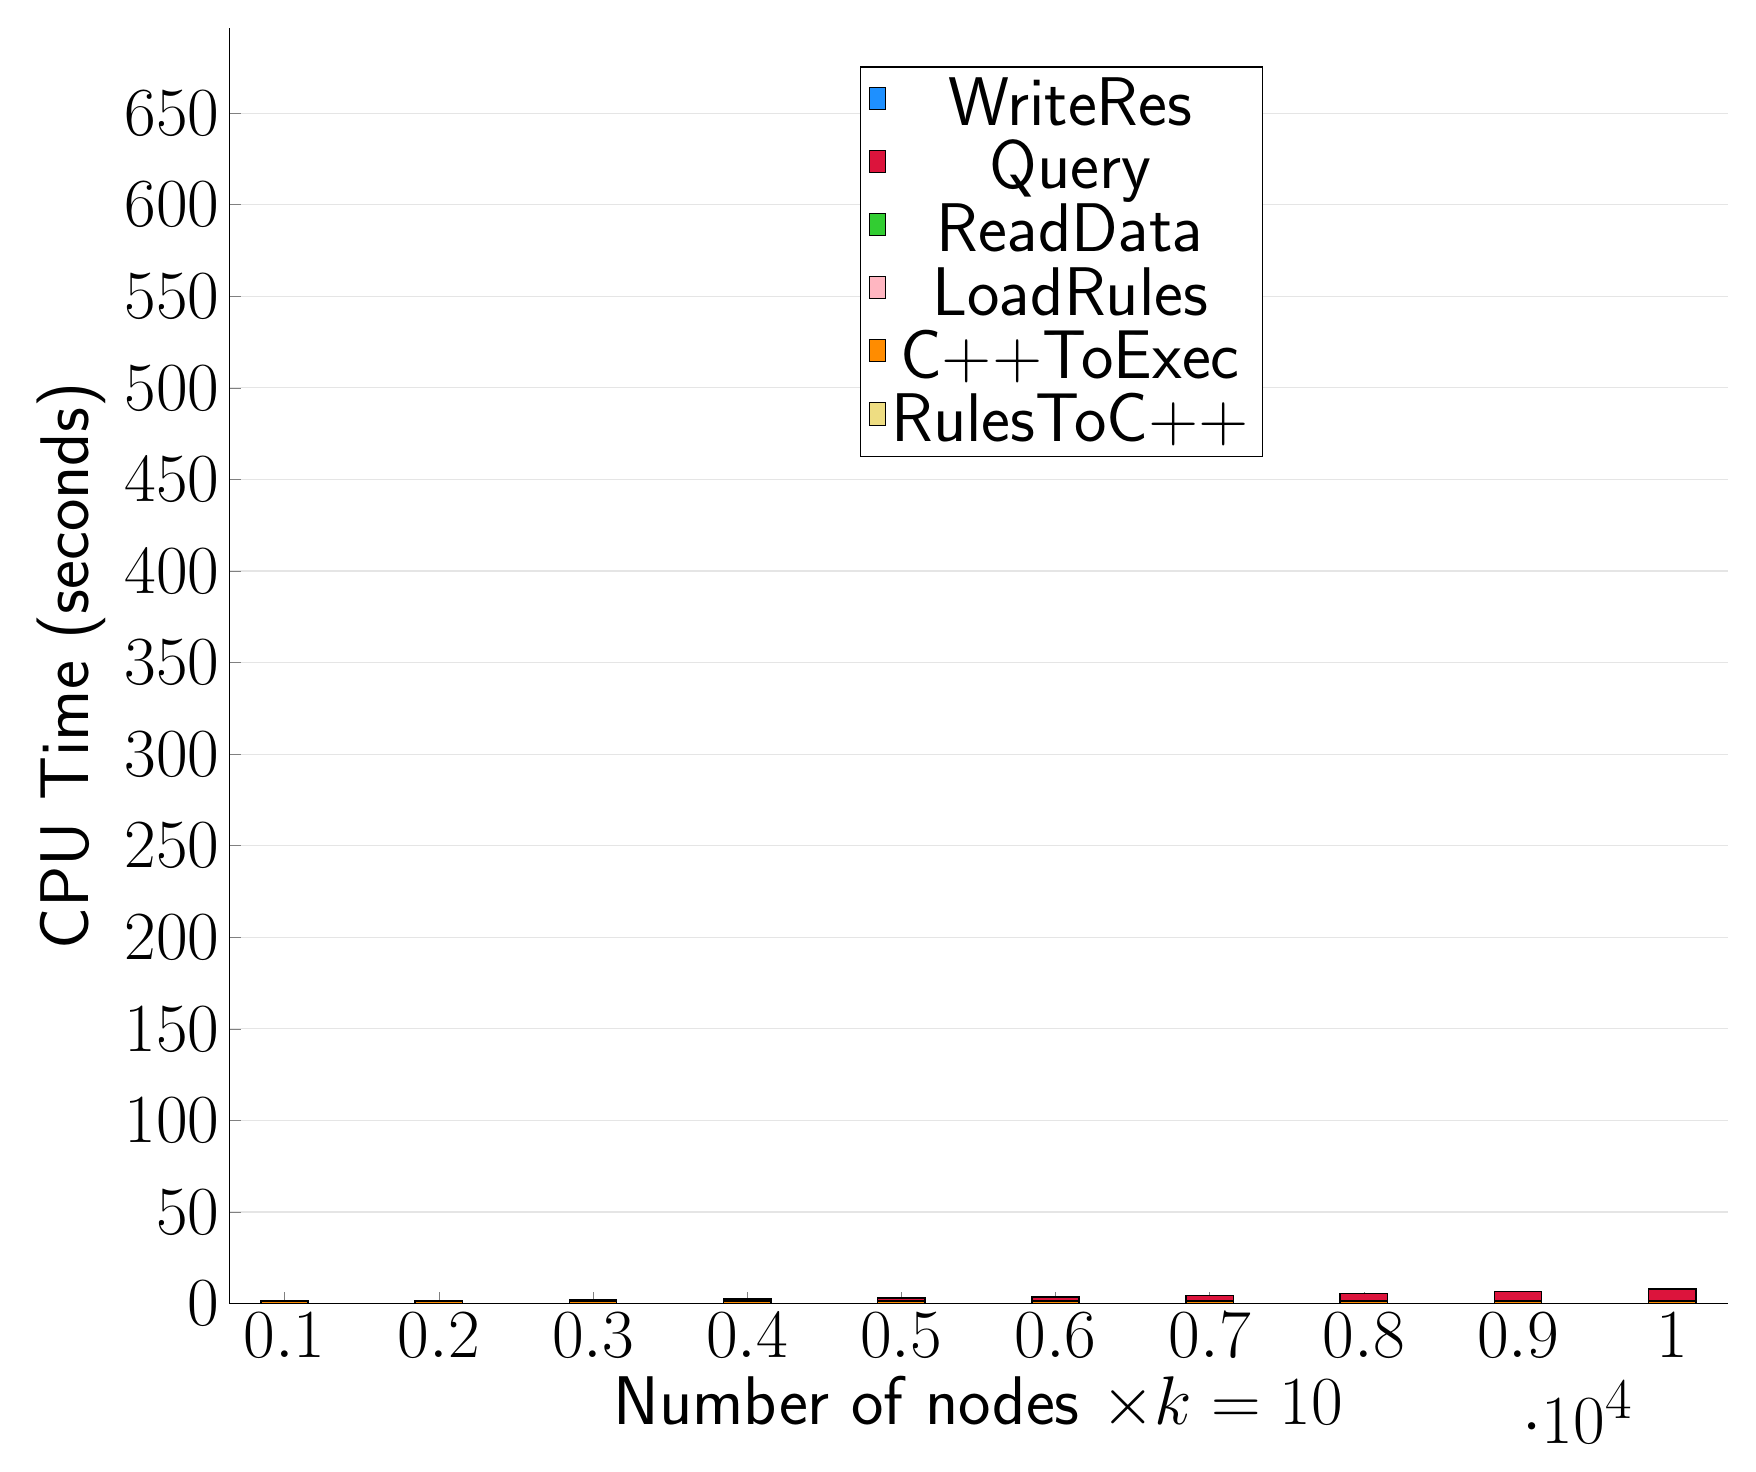
\begin{tikzpicture}
\begin{axis}[
   ybar stacked,
   width=1.7\textwidth,
   bar width=0.6cm,
   ymajorgrids, tick align=inside,
   major grid style={draw=gray!20},
   xtick=data,
   ymin=0, ymax=696.3414,
   axis x line*=bottom,
   axis y line*=left,
   enlarge x limits=0.04,
   legend style={
       at={(0.69, 0.97)},
       anchor=north east,
       legend columns=1,
       font=\Huge,
   },
   ylabel={CPU Time (seconds)},
   xlabel={Number of nodes $\times k=10$},
   label style={font=\Huge},
   tick label style={font=\Huge},
]
\addlegendimage{fill=DodgerBlue, draw=black, line width=0.2pt}
\addlegendentry{WriteRes}
\addlegendimage{fill=Crimson, draw=black, line width=0.2pt}
\addlegendentry{Query}
\addlegendimage{fill=LimeGreen, draw=black, line width=0.2pt}
\addlegendentry{ReadData}
\addlegendimage{fill=LightPink, draw=black, line width=0.2pt}
\addlegendentry{LoadRules}
\addlegendimage{fill=DarkOrange, draw=black, line width=0.2pt}
\addlegendentry{C++ToExec}
\addlegendimage{fill=LightGoldenrod, draw=black, line width=0.2pt}
\addlegendentry{RulesToC++}
\addplot +[fill=LightGoldenrod, draw=black, line width=0.55pt] coordinates {
(1000, 0.008000000000000002)
(2000, 0.010000000000000002)
(3000, 0.010000000000000002)
(4000, 0.008000000000000002)
(5000, 0.008000000000000002)
(6000, 0.006000000000000001)
(7000, 0.006000000000000001)
(8000, 0.004000000000000001)
(9000, 0.008000000000000002)
(10000, 0.008000000000000002)
};
\addplot +[fill=DarkOrange, draw=black, line width=0.55pt] coordinates {
(1000, 1.512)
(2000, 1.524)
(3000, 1.5260000000000002)
(4000, 1.5260000000000002)
(5000, 1.5240000000000002)
(6000, 1.532)
(7000, 1.5320000000000003)
(8000, 1.52)
(9000, 1.52)
(10000, 1.522)
};
\addplot +[fill=LightPink, draw=black, line width=0.55pt] coordinates {
(1000, 0.00014680000000000002)
(2000, 0.00015700000000000002)
(3000, 0.0001438)
(4000, 0.0001374)
(5000, 0.000151)
(6000, 0.0001526)
(7000, 0.0001396)
(8000, 0.000146)
(9000, 0.00015160000000000003)
(10000, 0.00013059999999999998)
};
\addplot +[fill=LimeGreen, draw=black, line width=0.55pt] coordinates {
(1000, 0.0039578)
(2000, 0.0071868)
(3000, 0.008899)
(4000, 0.011774000000000001)
(5000, 0.013603200000000001)
(6000, 0.016727)
(7000, 0.0172266)
(8000, 0.019974600000000002)
(9000, 0.0229098)
(10000, 0.022459)
};
\addplot +[fill=Crimson, draw=black, line width=0.55pt] coordinates {
(1000, 0.06844999999999998)
(2000, 0.23149900000000004)
(3000, 0.5222436)
(4000, 0.9444616)
(5000, 1.494782)
(6000, 2.1751980000000004)
(7000, 2.999714)
(8000, 3.9550899999999998)
(9000, 5.051918)
(10000, 6.298533999999999)
};
\addplot +[fill=DodgerBlue, draw=black, line width=0.55pt] coordinates {
(1000, 0.00022040000000000002)
(2000, 0.000232)
(3000, 0.00025120000000000003)
(4000, 0.00027860000000000005)
(5000, 0.00029240000000000006)
(6000, 0.000335)
(7000, 0.0002846)
(8000, 0.0003522)
(9000, 0.0003836)
(10000, 0.00039880000000000004)
};
\end{axis}
\end{tikzpicture}

\end{document}
